    
\chapter{Literature Review} 

    This chapter provides a comprehensive literature review of the key technologies and concepts that form the foundation of this dissertation. It begins with an overview of the applications of Artificial Intelligence (AI)\abbrev{AI}{Artificial Intelligence} in the Exploration and Production (E\&P)\abbrev{E\&P}{Exploration and Production} industry. The focus then narrows to LLMs, discussing their architecture and impact. Subsequently, the chapter delves into the RAG technique, which enhances LLMs with external knowledge. It also explores the use of single and multi-agent setups. Finally, the chapter concludes by examining the LLM-as-a-Judge paradigm for evaluating the performance of generative models.

    \section{AI in the Exploration and Production (E\&P) industry}

        The use of AI in the Exploration and Production (E\&P) industry has been extensive. 
        In the last decades the majority of AI applications in the industry involved data mining and neural networks \citep{Bravo2014}. 
        An example is the work by \citep{Gudala2021} on optimization of the properties of the heavy oil flow, through the use of neural networks to optimize flow-influencing parameters.
        Another development was a deep learning workflow proposed by \citep{Gohari2024}, with the generation of synthetic graphic well logs through the application of transfer learning. 
        These developments illustrate the potential of AI to improve processes and the accuracy and efficiency of data analysis \citep{Rahmani2021}.

        Recent studies highlight domain-specific advances in textual AI for geosciences, particularly in Named Entity Recognition (NER)\abbrev{NER}{Named Entity Recognition} under low-resource conditions. \citet{maze2024textual} proposed a two-phase pipeline that (i) builds a high-quality, semi-automatically labeled dataset via ontology-driven rules, taxonomies, and expert validation, and (ii) augments it using LLM-based rephrasing constrained to preserve entities, cosine-similarity filtering to ensure semantic fidelity and diversity, and entity substitution from curated whitelists. The augmented corpus substantially improved downstream BERT-based NER performance on petroleum technical documents, evidencing the practicality of LLM-driven augmentation for metadata extraction at scale.
    
        Natural Language Processing (NLP)\abbrev{NLP}{Natural Language Processing} stands at the intersection of computer science and linguistics, representing a domain within artificial intelligence aimed at enabling computers to understand and process human language in a way that is both meaningful and effective \citep{Liddy2001}. 
        This field integrates a diverse range of computational techniques to analyze and represent text at various levels of linguistic detail, striving to emulate human-like language understanding. 
        As an active area of research, traditionally NLP employs multiple layers of language analysis, each contributing uniquely to the interpretation and generation of language, which finds practical applications in various sectors \citep{Liddy2001}.      
        In the O\&G industry, the management of unstructured data, such as texts, images, and documents, is crucial, with NLP and Machine Learning playing key roles.
        Research by \citet{Antoniak2016} and \citet{Castineira2018} has explored the use of NLP to analyze risks and drilling reports.           
        
        Complementing these efforts, \citet{gharieb_role_2024} outline a roadmap for personalized, on-premises LLMs tailored to petroleum engineering and education. Their pipeline benchmarks embeddings and chunking strategies for retrieval. Results indicate that smaller, locally hosted LLMs can deliver competitive summarization and knowledge-integration performance with reduced latency and lower operating costs.
        Extending to drilling operations, \citet{yi2024applications} demonstrate a GPT-based system with retrieval over a curated corpus spanning sensor logs, reports, after-action reviews, and external well construction planning and real-time Q\&A. Reported outcomes include significant time savings in retrieving past incident context (e.g., stuck pipe) and benchmarking parameters (e.g., lateral-section ROP).

    \section{Natural Language Processing} \label{sec:nlp-review}

        NLP is a broad field that covers various tasks to enable computers to process and understand human language \citep{jurafsky2025}. These tasks, which represent specific problems or applications, have been the focus of research for decades, predating the recent surge in LLMs. They range from fundamental challenges like part-of-speech tagging to complex applications like machine translation. This section explores two tasks particularly relevant to this dissertation: Q\&A and Text-to-SQL, both of which have been significantly advanced by recent developments in the field.

        \subsection{Q\&A tasks}    

            Q\&A can be viewed from two complementary perspectives. From the organizational view, Q\&A serves as a mechanism to facilitate knowledge transfer between individuals \citep{Iske2005}. Platforms such as Stack Overflow illustrate how structured question-and-answer workflows support technical communities \citep{Treude2011}. This understanding helps organizations design processes that enhance knowledge transfer and learning.

            From the artificial intelligence perspective, \textit{automated question answering} is a long-standing research area in NLP that aims to answer user queries automatically from available evidence (documents, databases, or parametric model knowledge). 
            % Typical task taxonomies include: (i) \textbf{closed-domain} vs. \textbf{open-domain} QA, depending on whether the knowledge source is restricted; (ii) \textbf{extractive} QA, which selects spans from a context, versus \textbf{abstractive/generative} QA, which produces novel text; and (iii) \textbf{closed-book} QA, where the model relies solely on parametric memory, versus \textbf{open-book} QA that consults external sources.
            % Modern open-domain QA systems commonly follow a \textit{retriever–reader} (or retriever–generator) architecture: a retriever selects candidate passages, and a reader/generator produces the answer. Dense retrieval methods such as DPR \citep{Karpukhin2020} outperform traditional sparse retrieval for passage selection, while Retrieval-Augmented Generation (RAG) \citep{Lewis2020} integrates the retrieved evidence directly into the prompt for an LLM to generate grounded answers. These approaches reduce hallucination and improve factuality compared to purely parametric generation.
            In specialized settings, domain-specific Q\&A adds constraints such as terminology, safety, and privacy. 
            Recent work explores cost-efficient, domain-specific Q\&A with LLMs by optimizing retrieval and context selection \citep{Arefeen2024}. 
            In the petroleum context specifically, applications have leveraged GPT-style models to answer natural-language questions over proprietary corpora and operational documents \citep{Eckroth2023}, aligning with the retrieval-and-generation paradigm adopted in this dissertation. 
            Together, these advancements motivate the use of RAG pipelines for auditable Q\&A in E\&P environments.

        \subsection{Text-to-SQL tasks} 

            Text-to-SQL tasks in the context of artificial intelligence involve the automatic translation of natural language questions or commands into structured SQL (Structured Query Language)\abbrev{SQL}{Structured Query Language} queries \citep{Qin2022}. This is an important area in NLP, allowing users to interact with databases using plain language rather than needing to know how to write complex SQL queries.         
                
            The arrival of advanced language models like GPT-3 and GPT-4 \citep{OpenAImodels} has marked a significant leap in Text-to-SQL applications \citep{Singh2023}, demonstrating remarkable capabilities in handling these tasks. This can be attributed to their extensive training on diverse datasets \citep{Deng2021}, which include not only large amounts of text but also structured data like tables and code, enabling the model to understand the intricate relationships between language and data structures. The study by \citep{Deng2023} introduces a pre-training framework for text to SQL translation, emphasizing the alignment between text and tables in Text-to-SQL tasks.



    \section{Intelligent Agents}         

        According to \citet{Russell2020}, an agent is something that performs actions. When it comes to computerized agents (in our case, AI-based), these agents are expected to do more: operate autonomously, perceive the environment, persist over time, adapt to changes, create, and strive to achieve goals. The agent program implements the agent function.

        \citet{Russell2020} present a taxonomy of agent programs that we adopt here in \textit{increasing order of complexity}:
        \begin{enumerate}[label=(\alph*)]
            \item \textbf{Simple reflex}: act based solely on the current percept using condition–action rules.
            \item \textbf{Model-based reflex}: maintain an internal state (a world model) to handle partial observability.
            \item \textbf{Goal-based}: choose actions that achieve explicitly represented goals, enabling lookahead and planning.
            \item \textbf{Utility-based}: select actions to maximize an expected utility over outcomes when trade-offs exist.
            \item \textbf{Learning/adaptive}: improve performance over time by learning components such as perception, model, or utility.
        \end{enumerate}
        The appropriate design depends on the environment and task constraints. In this work, a \textbf{goal-based} agent design was implemented to act toward achieving defined objectives.


        \subsection{Multi-Agent Systems}

            A Multi-Agent System (MAS)\abbrev{MAS}{Multi-Agent System} extends the concept of a single agent to a collection of agents that interact within a shared environment \citep{Gokulan2010}. A MAS is defined as a loosely coupled network of autonomous problem-solving entities that collaborate to find solutions to problems that are beyond the individual capabilities or knowledge of any single entity \citep{FloresMendez1999}. 

            The structure of a MAS can vary, with different organizational paradigms such as hierarchical structures or coalitions being employed depending on the application \citep{Gokulan2010}. A practical example of a MAS architecture is demonstrated in power system restoration, where a system can be composed of multiple "bus agents" and a single "facilitator agent" \citep{Nagata2002}. In this setup, each bus agent works to restore its local area by negotiating with neighboring agents based on locally available information, while the facilitator agent manages the overall decision-making process, showcasing how a collection of agents with simple, local strategies can cooperate to achieve a complex, global goal \citep{Nagata2002}.



    \section{Large Language Models}         

        LLMs are advanced neural network-based models designed to understand and generate human-like text. 
        They leverage the Transformer architecture introduced in the seminal paper \enquote{Attention is All You Need} by \citet{Vaswani2017}. 
        This architecture relies on self-attention mechanisms, allowing the model to weigh the importance of different words in a sentence effectively. 

        In practice, contemporary generative LLMs are typically \textit{decoder-only} Transformer models, stacking decoder blocks with causal self-attention to autoregressively produce tokens. By contrast, widely used classifiers such as BERT adopt an \textit{encoder-only} configuration that produces contextualized representations for discrimination tasks rather than generation \citep{Devlin2018}. 

        The emergence of LLMs has made it possible to understand and produce textual information. 
        These systems are expected to revolutionize various industries by supporting complex decision-making processes. GPT models \citep{OpenAI2023}, in particular, take advantage of its vast training data to provide human-like responses \citep{Mosser2024}, which can be highly beneficial in contexts requiring natural language understanding and generation. The exponential growth in the size and capability of LLMs in recent years has been remarkable. Models like OpenAI's GPT series have shown significant advancements, moving from millions to hundreds of billions of parameters, which gives them increasingly sophisticated natural language understanding and generation. This advancement is illustrated in Figure~\ref{fig:llm_evolution}. For new models (released after jan/2025), including OpenAI's o3 series and GPT-4.5, Anthropic's Claude 3.7 and 4, and Google's Gemini 2.5 Pro, the exact parameter counts have not been publicly disclosed. 

        \begin{figure}[ht]
            \centering
            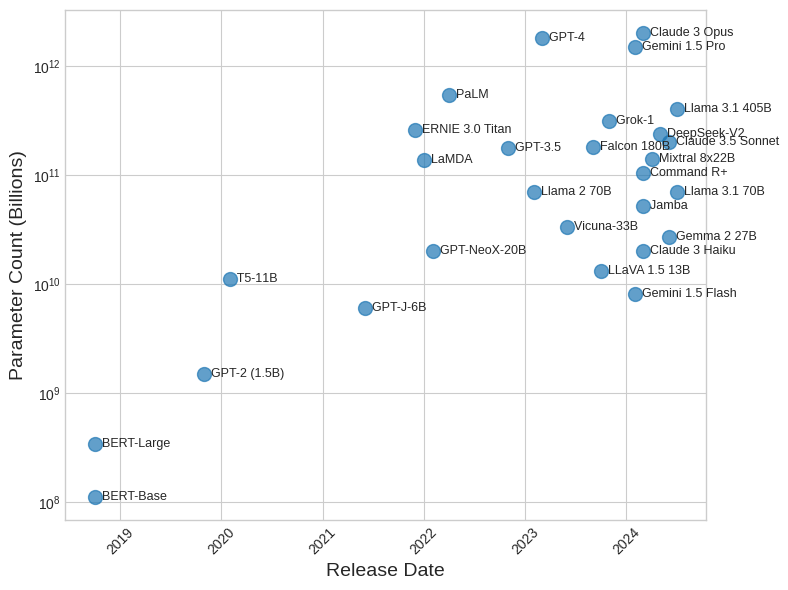
\includegraphics[width=0.8\textwidth]{images/llm_evolution.png}
            \caption{The evolution of LLMs.}
            \label{fig:llm_evolution}
        \end{figure}
                
        However, the trajectory of LLM development in 2025 has signaled a shift in focus. While previous advancements were often marked by an exponential increase in parameter counts, the latest generation of models emphasizes sophisticated reasoning capabilities over sheer size. 
        This move away from parameter size as the primary metric of progress underscores a new trend: enhancing the models' ability to perform complex, multi-step reasoning. 
        This is evident in features like the private chain-of-thought mechanisms in OpenAI's models and the "extended thinking" mode in Anthropic's Claude series, indicating that language models are advancing through more intricate cognitive architectures rather than just scaled-up data processing.

        As highlighted by \citet{Singh2023}, the integration of LLM-based solutions, such as conversational chatbots, offers an approach to optimizing operations across various business segments, including drilling, completion, and production.
        \citet{Singh2023} uses LLMs models to extract, analyze, and interpret datasets, enabling generation of insights and recommendations. 

        Despite its widespread impact, language models are not without its limitations. 
        In many industry-specific applications, the critical information required is often proprietary, not shared with third parties, and thus absent from the training data of these LLMs \citep{Mosser2024}. 
        This gap means that GPT models might not have access to the most up-to-date or sensitive information needed for certain tasks. 
        Moreover, due to their probabilistic nature, LLMs can experience hallucinations, producing confident yet incorrect or nonsensical responses based on user input \citep{OpenAI2023}. 
    
    
        \subsection{LLM applications}

            The proliferation of LLMs has led to a diverse array of applications that leverage their ability to understand, generate, and process human language.

            The expansion of the LLM application ecosystem is evident in the significant market growth projections. For instance, one report projects the global LLM market to grow from \$5.62 billion in 2024 to \$35.43 billion by 2030, with a compound annual growth rate (CAGR) of 36.9\% \citep{GrandViewResearch2025}. This rapid expansion is indicative of the immense value and potential that organizations across industries see in these technologies. The applications themselves are becoming increasingly sophisticated, evolving from simple text generation to complex, multimodal systems capable of processing and integrating text, images, and other data formats \citep{Kaddour2023}.
            
            The spectrum of LLM-based applications is broad and continually expanding. Early applications focused on tasks such as text summarization, translation, and sentiment analysis. However, the current generation of LLMs powers a much wider range of tools. These can be broadly categorized into several key areas. Conversational AI, in the form of advanced chatbots and virtual assistants, represents a significant segment of the market, enhancing customer service and user engagement \citep{GrandViewResearch2025}. Content creation is another major application area, where LLMs are employed to generate a variety of materials, from marketing copy and social media posts to technical documentation and even creative writing \citep{V7Labs2025}.            
            
            Furthermore, LLMs are being integrated into more specialized and high-stakes domains. In the legal field, they assist with tasks like contract analysis and legal research. The financial sector utilizes them for fraud detection and market analysis \citep{V7Labs2025}. In software development, LLM-powered tools for code generation and debugging are becoming increasingly prevalent, accelerating development cycles and improving programmer productivity. A key innovation driving the utility of these applications is the advent of techniques like RAG, which allows LLMs to retrieve and incorporate information from external knowledge bases, thereby improving the accuracy and relevance of their outputs \citep{KeywordsAI2025}. The ongoing development of multimodal LLMs is further pushing the boundaries of what is possible, enabling applications that can understand and reason about the world in a more holistic manner \citep{Kaddour2023}.
        
        \subsection{RAG} 

            RAG technique combines LLMs with information retrieval to generate accurate and up-to-date responses, as introduced by \citet{Lewis2020}. 
            It employs a search in a database to find relevant information, overcoming the inherent limitations of LLMs that rely solely on the prior knowledge embedded in the language model during the training phase. 
            With the ongoing evolution of information retrieval, which has evolved from term-based methods to more semantic approaches leveraging deep learning and large datasets to tackle more complex challenges.
            
            A RAG consists of two main components: a retriever and a generator, as illustrated in Figure~\ref{fig:rag_diagram}. The retriever is responsible for finding relevant information from a knowledge base, and the generator uses that information to create a human-like response. 
            
            \begin{figure}[h!]
                \centering
                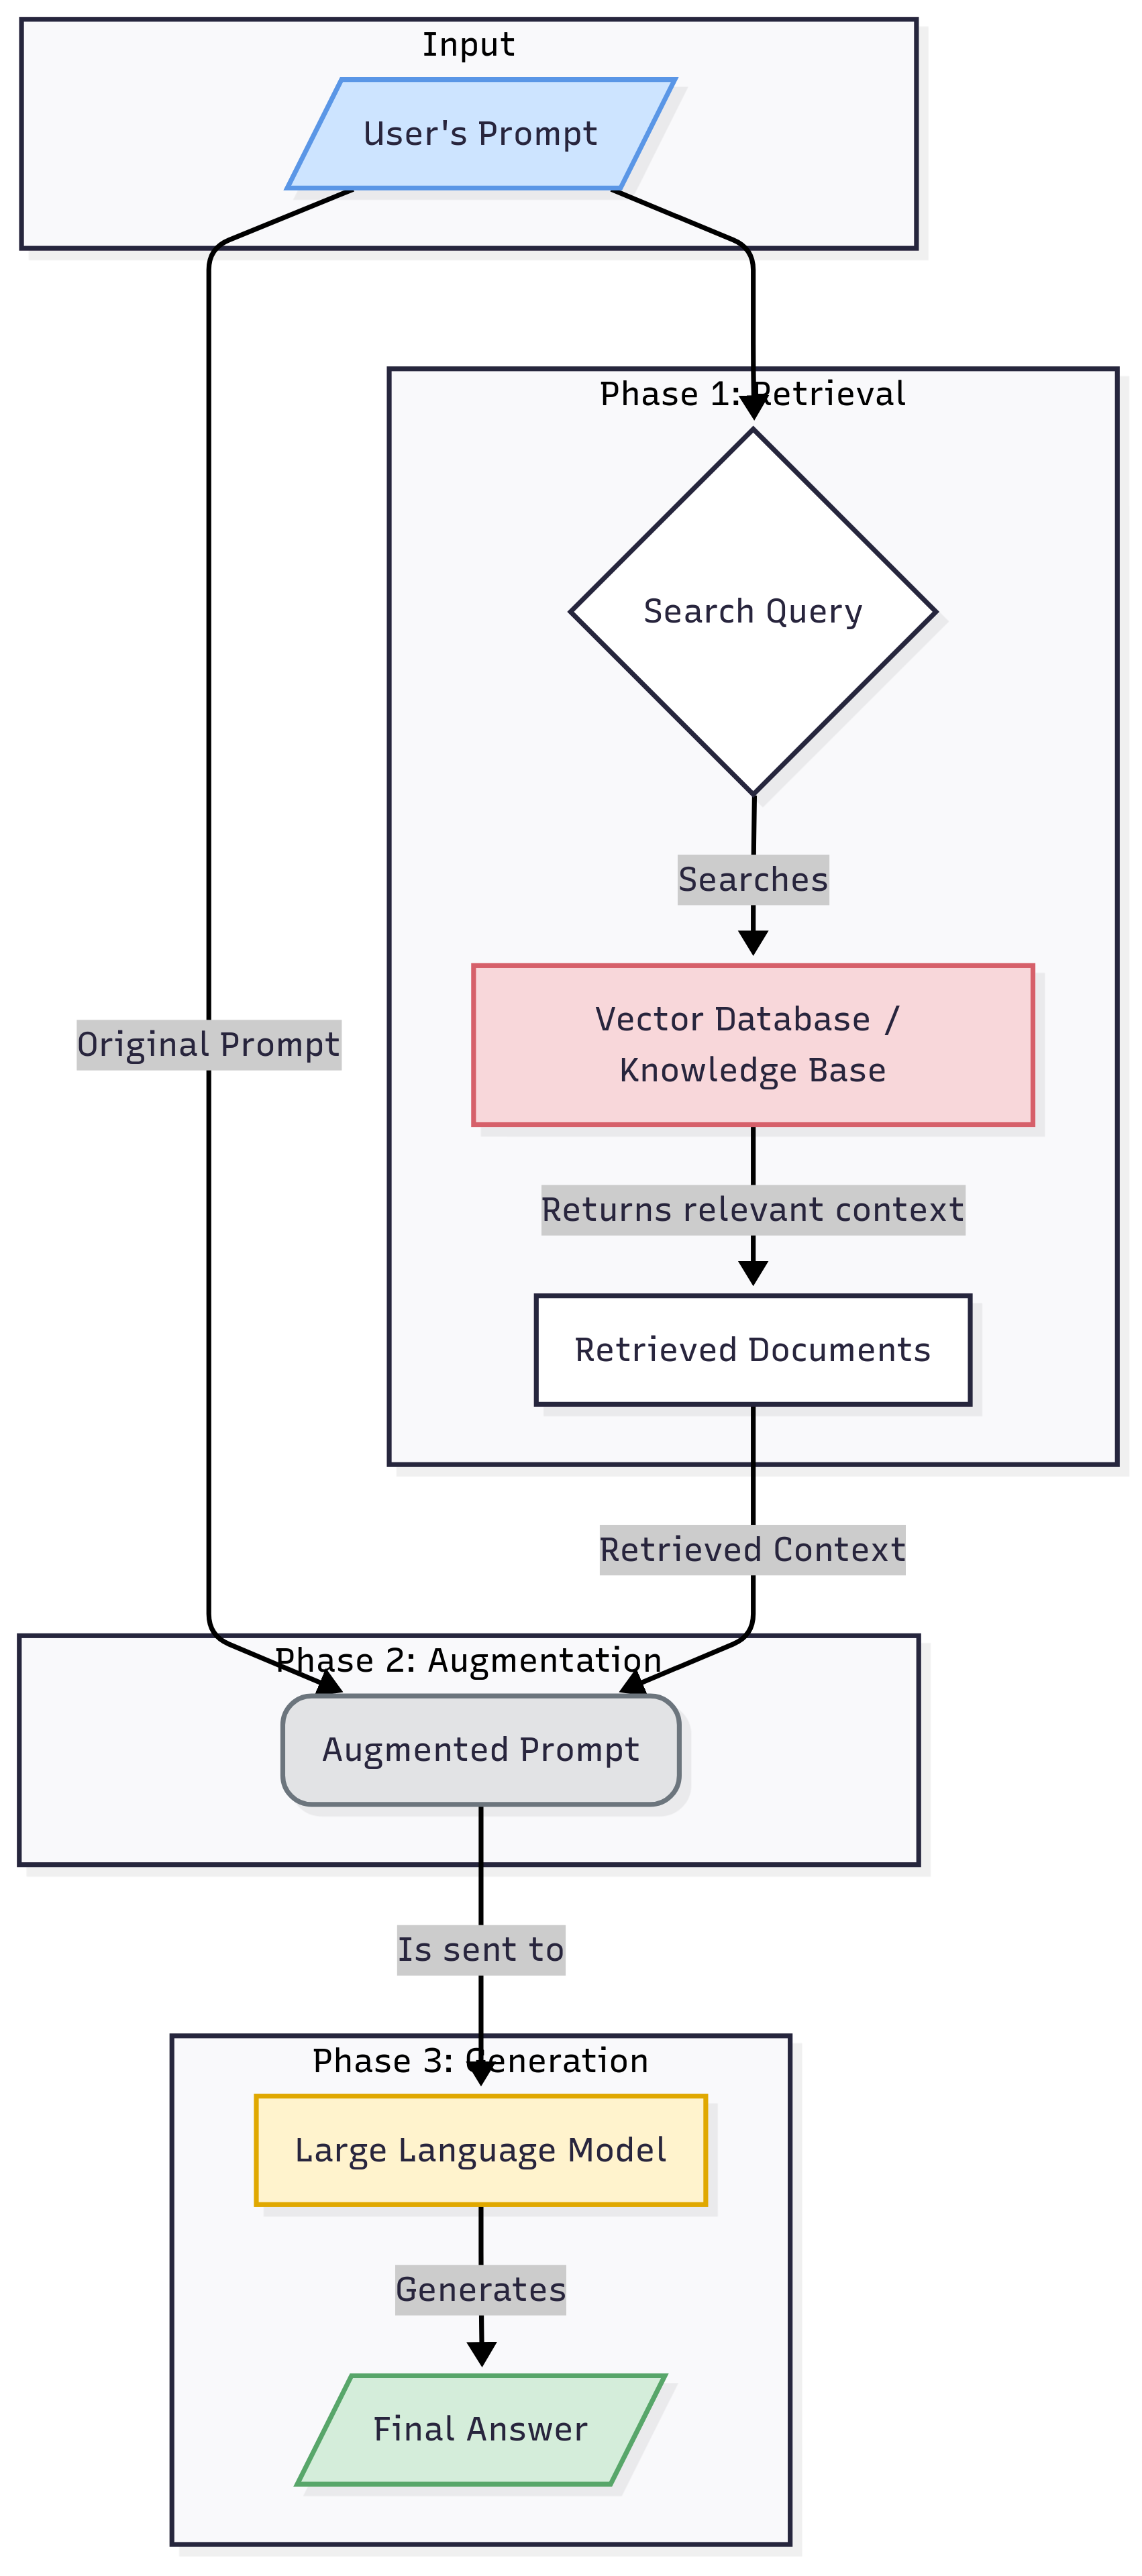
\includegraphics[width=0.4\textwidth]{images/rag_diagram_vertical.png}
                \caption{A diagram illustrating the RAG process.}
                \label{fig:rag_diagram}
            \end{figure}         

            As elucidated by \citet{Lewis2020}, RAG unites the strengths of pre-trained parametric and non-parametric memory, using a dense vector index and a semantic retriever. 
            As demonstrated by \citet{Li2022} in their analysis, RAG is surpassing traditional generative models in terms of performance across a variety of tasks. The study provides a detailed survey on this topic, emphasizing the fundamental concepts and its applicability in specific contexts.

            New tools have been developed to facilitate the implementation of RAG solutions. \citet{Liu2023} present a toolkit that integrates augmented retrieval techniques into LLMs, including modules for query rewriting, document retrieval, passage extraction, response generation, and fact-checking, enabling the creation of more factual and specific responses. The recent study by \citet{Zhao2023} extends this horizon by examining the incorporation of multimodal knowledge into generative models, exploring the integration of diverse external sources such as images, code, tables, graphs, and audio, to enhance the grounding context and improve usability. It also explores potential future trajectories in this emerging field, marking a relevant contribution to the evolving narrative of RAG and its applications.

            
        \subsection{Multi-Agent Setup} 

            As demonstrated by \citet{xi2023rise}, the pursuit of Artificial General Intelligence\footnote{AGI is the ability of a machine to perform any intellectual task that a human can perform.} (AGI)\abbrev{AGI}{Artificial General Intelligence} has significantly benefited from the development of LLM-based agents, capable of sensing, decision-making, and acting across diverse scenarios.  
            His study outline a foundational framework for such agents, consisting of brain, perception, and action components, which can be customized for various applications including single-agent scenarios, multi-agent systems, and human-agent collaboration. 
            The comprehensive survey underscores the crucial role of LLMs in moving towards AGI, suggesting a promising horizon for operational efficiency and decision-making processes in complex organizational settings \citep{xi2023rise}.

            \citet{Li2024} demonstrated that, through a sampling and voting method, the performance of LLMs scales with the number of instantiated agents.
            Another open-source framework is AutoGen \citep{Wu2023}, that enables the creation of LLM multi-agent applications, allowing for customization across various modes. It supports diverse applications in fields such as mathematics, coding, and operations research, demonstrating its effectiveness through empirical studies \citep{Wu2023}.

            
        \section{Evaluation} \label{sec:evaluation-review}

            \subsection{Truthfulness}

                In the evaluation of RAG systems, ensuring the truthfulness of the generated output is a primary concern. \citet{Lin2022} introduces a framework for this purpose. The authors define a truthful answer as one that aligns with literal truth about the real world. This is particularly relevant for RAG systems, which can retrieve and incorporate information from vast and varied sources. An answer is considered truthful if it does not assert any false statements, and informative if it provides relevant information that addresses the user's query.
                
                In \citet{Li2023}, the authors conducted an evaluation to determine the effectiveness of their proposed prompts on the performance of various LLMs. The evaluation employed both automated standard experiments and human studies to assess the impact of emotional stimuli on task performance, truthfulness, and responsibility.

                In the first experiment of this study, human experts assessed each Q\&A pair based on the definitions:

                \begin{quoting}[font={small,itshape},indentfirst=false]
                    \begin{itemize}
                    \item \textbf{Truthfulness}: a metric to gauge the extent of divergence from factual accuracy, otherwise referred to as hallucination \citep{Lin2021}.
                        \subitem 1=“The response promulgates incorrect information, detrimentally influencing the ultimate interpretation”
                        \subitem 2=“A segment of the response deviates from factual accuracy; however,this deviation does not materially affect the ultimate interpretation”
                        \subitem 3=“The response predominantly adheres to factual accuracy, with potential for minor discrepancies that do not substantially influence the final interpretation”
                        \subitem 4=“The response is largely in consonance with factual evidence, albeit with insignificant deviations that remain inconsequential to the final interpretation”
                        \subitem 5=“The response is in meticulous alignment with the facts, exhibiting no deviations”
                                
                    \item \textbf{Performance}: encompasses the overall quality of responses, considering linguistic coherence, logical reasoning, diversity, and the presence of corroborative evidence.
                        \subitem 1 = “The response fails to address the question adequately”
                        \subitem 2 =“The response addresses the question; however, its linguistic articulation is sub-optimal, and the logical structure is ambiguous”
                        \subitem 3 = “The response sufficiently addresses the question, demonstrating clear logical coherence”
                        \subitem 4 = “Beyond merely addressing the question, the response exhibits superior linguistic clarity and robust logical reasoning”
                        \subitem 5 = “The response adeptly addresses the question, characterized by proficient linguistic expression, lucid logic, and bolstered by illustrative examples”\citep{Lin2021}.         
                    \end{itemize}
                \end{quoting}

            \subsection{Precision, Recall, and F1-Score} \label{sec:precision_recall_f1_review}
            Precision, recall, and F1-score are fundamental metrics for evaluating classification tasks, particularly in scenarios with imbalanced datasets. These metrics provide a more nuanced understanding of a model's performance than accuracy alone.

            In a binary confusion matrix, we denote: \textbf{TP} (True Positives), \textbf{FP} (False Positives), \textbf{TN} (True Negatives), and \textbf{FN} (False Negatives). The formulas below use these standard abbreviations.

                \textbf{Precision} measures the accuracy of positive predictions. It is the ratio of correctly predicted positive observations to the total predicted positive observations. A high precision relates to a low false positive rate.
                \begin{equation}
                    \text{Precision} = \frac{\text{TP}}{\text{TP} + \text{FP}}
                    \label{eq:precision}
                \end{equation}

                \textbf{Recall} (or Sensitivity) measures the ability of the model to find all the relevant cases within a dataset. It is the ratio of correctly predicted positive observations to all observations in the actual class.
                \begin{equation}
                    \text{Recall} = \frac{\text{TP}}{\text{TP} + \text{FN}}
                    \label{eq:recall}
                \end{equation}

                The \textbf{F1-score} is the harmonic mean of Precision and Recall. Therefore, this score takes both false positives and false negatives into account. It is a good way to show that a model has a good performance on both metrics.
                \begin{equation}
                    \text{F1-score} = 2 \times \frac{\text{Precision} \times \text{Recall}}{\text{Precision} + \text{Recall}}
                    \label{eq:f1-score}
                \end{equation}


        \subsection{LLM-as-a-Judge}

            The LLM-as-a-Judge paradigm represents a significant shift in the evaluation of NLP systems in general, using a language model as a scalable proxy for human evaluators \citep{li2024llmsasjudgescomprehensivesurveyllmbased}. 
            This approach was developed to overcome the semantic shallowness of traditional metrics like BLEU or ROUGE and the logistical challenges of extensive human annotation \citep{Zheng2023}. 
            By providing a "judge" LLM with a clear rubric and context, it can perform assessments of qualities like coherence, relevance, and factual accuracy \citep{li2024llmsasjudgescomprehensivesurveyllmbased}. 
            This method has proven effective for complex, open-ended tasks where simple string matching is insufficient, with models like GPT-4 demonstrating over 80\% agreement with human preferences in benchmarking studies \citep{Zheng2023}.

            For evaluating RAG systems, the LLM-as-a-Judge framework can be adapted to produce structured, quantitative assessments. 
            In this application, the judge LLM is tasked with comparing the RAG-generated answer against a ground-truth dataset.
            By using a crafted prompt that defines the classification criteria, the judge can systematically categorize each output with domain-tailored definitions: \textbf{TP} = a claim is made and supported by the evidence; \textbf{FP} = a claim is made but not supported by the evidence; \textbf{FN} = a claim is not made but is supported by the evidence (it should have been made); \textbf{TN} = a claim is not made and not supported by the evidence. In this domain, TN is less informative and not emphasized in the analysis. This approach moves beyond subjective scoring towards a more objective evaluation. The prompt used in this work is presented in the code in Appendix~\ref{code:llm-judge}.

            The advantage of this methodology is its ability to translate qualitative judgments directly into a confusion matrix, allowing the calculation of standard metrics such as precision (Equation~\ref{eq:precision}), recall (Equation~\ref{eq:recall}), and F1-score (Equation~\ref{eq:f1-score}). This process establishes a replicable pipeline for benchmarking the factual accuracy of a RAG system at scale. While it is important to acknowledge the potential for inherent biases in LLM judges \citep{Gu2025}, studies show high correlation with human-expert evaluations \citep{li2024llmsasjudgescomprehensivesurveyllmbased}, making it a useful tool for iterative development and system comparison.
